\documentclass[12pt]{article}
\usepackage{graphicx,booktabs,setspace,listings}
\doublespacing
\usepackage[np]{numprint}
\npstyleenglish
\usepackage{hyperref}
\begin{document}

	\title{16S RNA Sequencing Data Management using SQLite}
	\author{Xu Junjie, Kevin}
	\date{June 2014}
	\maketitle
	\begin{abstract}
		16S Ribosomal RNA Sequencing is used extensively in analzying bacterial
		phylogeny and taxonomy. This project attempts to streamline the 16S sequencing
		pipeline using local file databases to replace multiple flat sequence files used
		in the pipeline, to ease logistical burdens on the researcher and enable 
		greater metadata analysis and accountability of experiments.
	\end{abstract}
	\tableofcontents
	\section{Introduction} % (fold)
	\label{sec:introduction}
	The 16S small subunit of bacterial ribosomes are highly gene sequences found in all bacteria, which means that the differences within the 16S RNA profiles can be used as an analogue for species identity. Since the 16S gene contains both highly conserved and highly variable regions all interspersed together,
	the highly conserved regions can be amplified using PCR (Polymerase chain reaction), while the variable regions are used to classify the organism. HTS (High Throughput Sequencing) using Illumina sequencers are then used to sequence the PCR products from the prior step.

	The output from HTS forms the start of the computational pipeline. In the preprocessing stage, poor quality reads are filtered and trimmed. 
	Chimeras\footnote{a single organism composed of genetically distinct cells} and non-bacterial 16S reads are then removed. 
	The pipeline then attempts to produce phylogenetic classification through the use of classification based on sequence similarity (i.e. OTU Analysis). By comparing the filtered output from HTS against the already existing taxonomies of over 2 million species, the genus, family, and order of the sample can be determined.

	%The classifier can fail for various reasons: for example, the majority of bacterial species have not been identified or sequenced, the 16S reads are usually too short for accurate classification. In those cases, groups of highly similar sequences are grouped into OTUs (Operational Taxonomic Unit) that can be analyzed for quantitative differences in communities between the sequenced samples.

	%The project utilizes a computational approach due to the large amount of raw sequencing data that is created from the PCR amplification process. The variability of results is further affected by the OTU Analysis stage, where prior parameters can affect the analysis outcome. Using a computational approach would allow the change of various parameters, in order to quantitate the effects of those parameter changes.

	The majority of the pipeline is executed on the University of Oregon’s ACISS High-Performance Supercomputer Cluster, and utilizes PBS scripts (normal shell scripts with extra variables defined to manage job resources) to execute the different stages of the pipeline.

	(flowchart placeholder)

	The FASTQ output produced by the Illumina sequencer is run through the preprocessing stage of filtering, trimming, and demultiplexing. The PBS script for the preprocessing stage calls on the Demultiplexer, a python script written by Rodger Voelker, which removes the primer attached to the sequences during the amplification process, and attaches barcodes (signifying sample origin) to both ends of the paired-end reads in the FASTQ file. After demultiplexing, the pipeline proceeds to use Trimmomatic v0.32, an open source tool to trim poor quality feeds from the reads. It uses a sliding window trimming, that cuts out sequences when the average quality within a window falls below a certain threshold. 
	Bowtie 2.1.0 is used to align the reads to existing mitochondrial and phiX sequences and to remove them.
	
	Pip (Pipeline Interface Program) was developed to explore the feasibility of 
	storing 16S Ribosomal RNA Sequencing pipeline work products in a SQLite database.
	The project began on the preprocessing (primer splitting, trimming, quality filtering) 
	stages of the pipeline, preparing the work products from the raw sequencing 
	data produced by the Illumina NGS machines to be fed into the analysis (clustering, alignment, phylogenic inference) 
	stages. 
	
	% section introduction (end)
	\section{Data Management} % (fold)
	\label{sec:data_management}
	Management of data in a pipeline is conceptually divided into four tasks: 
	creating semantic structure within the database; storing sequence data in compressed form;
	transforming stored data into formats required by tools in the pipeline; logging
	settings and parameters of transformations and related metadata.
	
	As the first stage in a 16S pipeline, Pip combines primer sequences, barcodes, 
	offsets, and raw Illumina NGS (Next-Gen Sequencing) FASTQ files into a single, 
	compressed file that acts as a logical container for the experiment. Pip 
	encapsulates the data with adapters to transform the compressed data into 
	usable input for subsequent stages, and provides metadata logging.

	\subsection{Semantic Database Structure} % (fold)
	\label{sub:semantic_database_structure}
	Instead of juggling multiple input files such as raw Illumina FASTQ sequences,
	barcodes, and offsets, Pip creates several SQLite tables which impart a well-defined
	semantic structure to the data and contains them within a single file.
	
	A Pip database is initialized with six tables:
	
	\begin{description}
		\item[primer] holds all primer sequences used in the experiment
		\item[offset] randomized offsets to aid 16S sequencing
		\item[barcode] experiment identifier
		\item[log] stores all metadata related to data, experiment, or pipeline
		\item[read1] stores the first part of paired-end sequence data
		\item[read2] stores the second part of paired-end sequence data
	\end{description}
	
	The primer, offset, and barcode tables links information about the experiment 
	to the actual sequences to be stored in the read1 and read2 tables.
	
	Every operation done in Pip can be stored as metadata in the log table, providing a
	detailed record of all settings and parameters used at the time of operation. 
	Results of OTU Analysis can be affected by parameters used by the tools upstream
	in a pipeline, thus having a reliable record of operations and transformations
	to the data will aid in analysis downstream.

	% subsection database_structure (end)

	\subsection{Data Compression} % (fold)
	\label{sub:data_compression}
	FASTQ files generated by Illumina NGS machines have this general format:
	
	\lstset{
		numbers=right
	}
	\begin{lstlisting}
@HWI-ST0747:277:D1M96ACXX:6:1101:1232:2090 1:N:0:
GGATAGTACTAGGGTATCTAATCCTGTTTGCTCCCCACGCT...
+
ACCCFFDDFH#FHHIGIJJFJJJJJJJJJJJIIJJJGIJJG...
	\end{lstlisting}
	where line 1 is the \emph{defline} containing information about the Illumina
	Sequencer which produced the sequence, line 2 contains all the bases in the 
	sequence, line 3 is the separator between the sequence and quality scores, and 
	line 4 contains the corresponding quality score for each of the bases in the 
	sequence. Each character in the file ias an ASCII character taking up 8 bits. 
	The format uses five characters to represent the four DNA-bases (A - adenine, T - thymine,
	C - cytosine, G - guanine) and N to represent an errorneous read. Each base is paired
	with a quality score that has 42 values (0 to 41). Compression works by representing
	each base with an integer range (A: 0 to 49, T: 50-99, C: 100-149, G: 150-199, N: 200-255)
	and adding the quality score to the beginning of that range. Thus, base `A' with a 
	quality score of `\#' (value 0) can be represented by the value 0, while base `G' with
	a quality score of `J' (value 41) can be represented by 191 (150 + 41). The resulting
	values fit within an 8-bit character, which is a 50\% reduction in space usage. 
	Since both compression and decompression require only addition operators, the scheme
	is fast and lossless.

	% subsection compression (end)
	
	\subsection{Data Transformation} % (fold)
	\label{sec:data_transformation}
	A central part of managing the sequence data in the 16S pipeline is the manipulation
	and transferring of sequences between the various tools. There is often a need
	to modify the structure or format of the data to fit the varying input requirements
	of those tools. Table~\ref{tab:expected_input} shows the various input formats that
	tools in the pipeline require.

	\begin{table}
		\centering
		\begin{tabular}{c|c}
		\hline
		Tool & Expected input format\\
		\hline
		Trimmomatic & FASTQ/Gzipped FASTQ\\
		\hline
		Bowtie2 & FASTQ/FASTA\\
		\hline
		QIIME & 454-FASTA/454-Quality Scores\\
		\hline
		\end{tabular}
		\caption{Expected input formats for various tools}
		\label{tab:expected_input}
	\end{table}

	Traditionally, the way to manage the various formats was to transform and store
	various copies of the data in multiple files. For example, the first stage of 
	the pipeline usually involves using Trimmomatic to filter poor quality reads 
	and to trim all the reads to a certain length. Doing this requires the user to
	provide 2 paired-end FASTQ sequence files to Trimmomatic, which will then produce
	5 output files: unpaired and paired sequences 1 and 2, and a trimming log. The 
	output files have sizes similar to the input, which results in the space usage
	nearly doubling after the first stage in the pipeline. Subsequent stages will
	then take the output of the first stage and create more output. Thus, both
	the number of files and their file size will increase very quickly due to the 
	number of stages within the 16S pipeline.
	
	Using a plug-in architecture, Pip can ``stream'' sequence data to tools in the
	pipeline without writing to disk. Pip uses UNIX Named Pipes to 
	feed data to tools such as Trimmomatic and Bowtie while simultaneously consuming the output
	they produce back into the database. UNIX Named Pipes allows programs to transfer
	data through memory instead of disk, and therefore do not require reading and
	writing to disk. However, named pipes appear as size zero, regular files on a filesystem,
	thus tools can read and write from those files without needing any changes
	to the software. In the case of Trimmomatic, Pip provides a named pipe to capture
	the contents of the trimming log, and uses the details within it (sequence number, 
	position of trim, number of characters trimmed) and stores them in a ``trimmed''
	table. Since this table only stores the sequences which were operated on, instead 
	of entire copies of the original sequences, the size increase of the Pip database
	after the first stage is almost negligible. Additionally, instead of needing to
	manage multiple output files and their naming, the data is now ready for the 
	next stage of the pipeline.
	% subsection data_flow_using_unix_pipes (end)
	% section data_management (end)

\section{Results} % (fold)
\label{sec:results}
Pip was benchmarked on a 2.7 GHz Intel Core i7 processor with 16GB of RAM, running
OS X 10.9. Table~\ref{tab:insertion_speeds} shows the time taken for the specified number
of sequence inserts into a new Pip database. Figure~\ref{fig:insertion_speeds} plots the
number of actual raw inserts per second into SQLite, showing consistent insertion 
rates between \np{96000} and \np{102000} raw inserts per second.

\begin{table}[h!]
\centering
\begin{tabular}{n{4}{2}|n{4}{2}}
	\toprule
 {Number of sequences (paired-end)} & {Time taken (seconds)} \\
 \midrule
 \np{500000} & 10.35 \\
 \np{1000000} & 19.57 \\
 \np{2000000} & 39.22 \\
 \np{4000000} & 78.67 \\
 \np{8000000} & 160.84 \\
 \np{16000000} & 319.38 \\
 \np{32000000} & 644.90 \\
 \np{64000000} & 1286.26 \\
 \bottomrule
\end{tabular}
\caption{Insertion speeds into SQLite using Pip}
\label{tab:insertion_speeds}
\end{table}

\begin{figure}[h!]
	\centering
	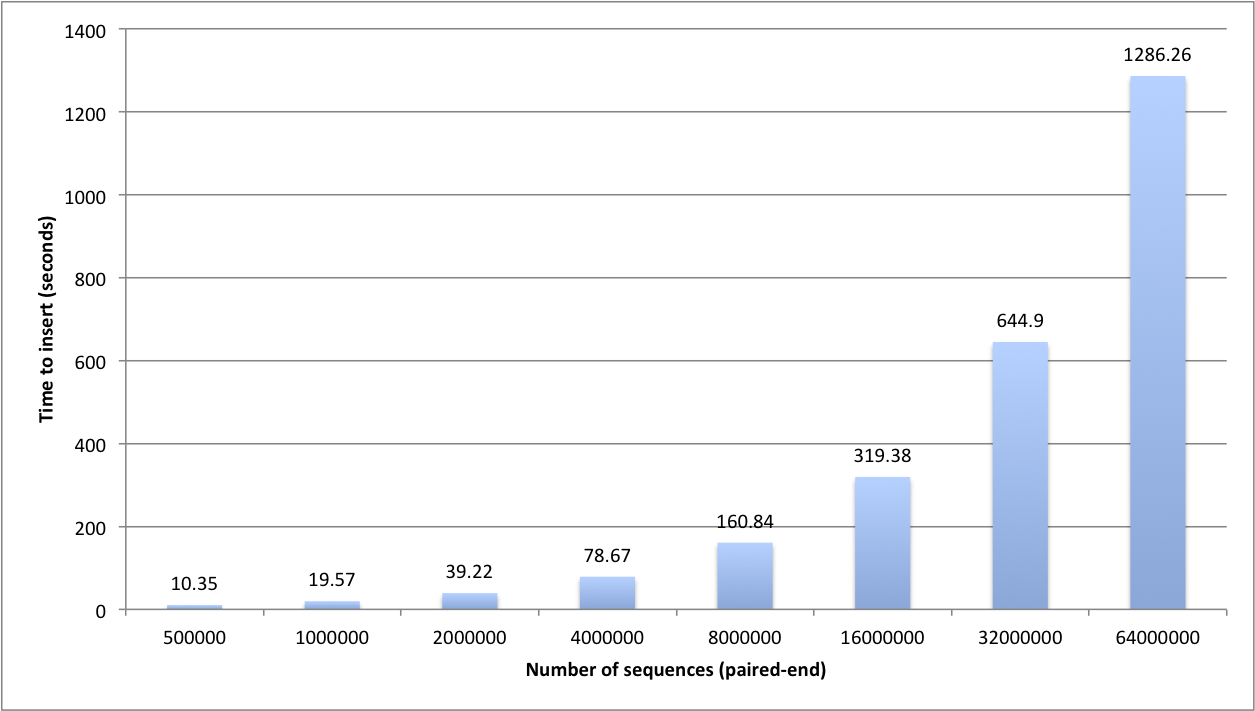
\includegraphics[width=\textwidth]{insertion_speed_chart}
	\caption{Inserts per second into SQLite using Pip}
	\label{fig:insertion_speeds}
\end{figure}
\newpage
Table~\ref{tab:filesizes} shows the size of the raw FASTQ sequence file compared to the resulting
database file after inserts. Figure~\ref{fig:filesizes} reveals a consistent
45\% reduction in file size after insertions.

\begin{table}[h!]
\centering
\begin{tabular}{n{0}{0}|n{6}{2}|n{6}{2}}
	\toprule
 {Number of sequences (paired-end)} & {Input FASTQ size (MB)} & {Pip database (MB)} \\
 \midrule
 \np{500000} & 371.40 & 206.90 \\
 \np{1000000} & 743.00 & 413.90 \\
 \np{2000000} & 1486.00 & 828.00 \\
 \np{4000000} & 3051.52 & 1699.84 \\
 \np{8000000} & 6082.56 & 3389.44 \\
 \np{16000000} & 12165.12 & 6789.12 \\
 \np{32000000} & 24350.72 & 13568.00 \\
 \np{64000000} & 48701.44 & 27146.20 \\
 \np{91000000} & 69754.88 & 35061.76 \\
 \bottomrule
\end{tabular}
\caption{Comparison of input file sizes against Pip database sizes}
\label{tab:filesizes}
\end{table}

\begin{figure}[h!]
	\centering
	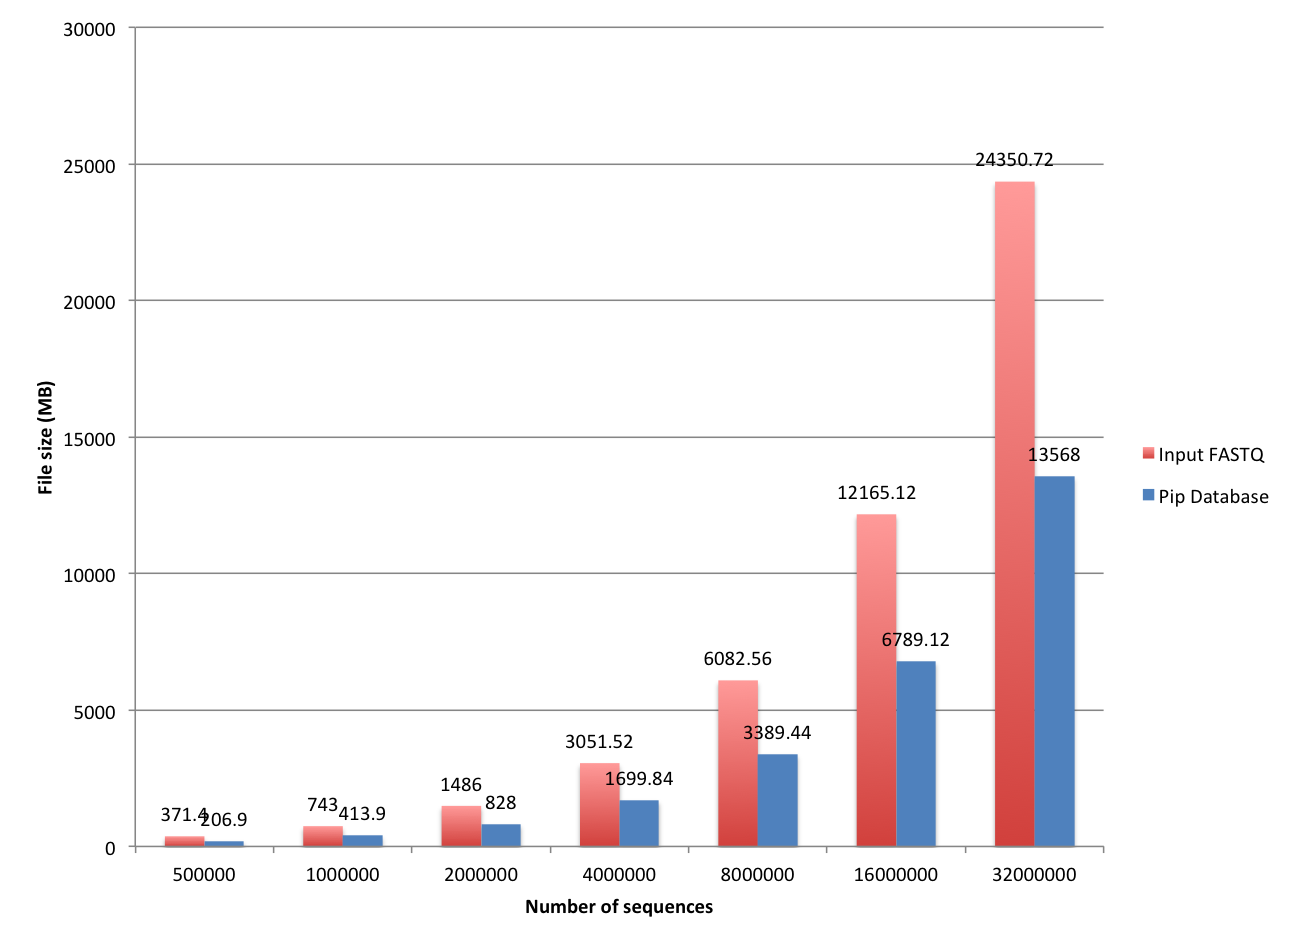
\includegraphics[width=\textwidth]{filesizes_chart}
	\caption{File sizes of Pip database against original FASTQ files}
	\label{fig:filesizes}
\end{figure}

\begin{table}[h!]
\centering
\begin{tabular}{c|n{6}{2}|n{6}{2}}
	\toprule
 {Pipeline Stage} & {Raw time (seconds)} & {Pip time (seconds)} \\
 \midrule
 Trimmomatic 1-thread & 46.43 & 22.89 \\
 Trimmomatic 2-thread & 25.96 & 23.58 \\
 Trimmomatic 4-thread & 26.05 & 23.77 \\
 Trimmomatic 8-thread & 26.46 & 23.21 \\
 \bottomrule
\end{tabular}
\caption{Time needed to process \np{500000} sequences through 16S pipeline stages with and without Pip}
\label{tab:streamspeed}
\end{table}

% section results (end)

%\section{Analysis and Applications} % (fold)
%\label{sec:analysis_and_applications}

% section analysis_and_applications (end)

\section{Conclusion} % (fold)
\label{sec:conclusion}
The use of Pip within the 16S pipeline shows promise in reducing the logistical
effort of researcher and interoperability headaches of multiple tools. Currently,
Pip operates on the first two tools of the 16S pipeline (Trimmomatic, Bowtie) and
shows promise. Pip can be extended to with tools later in the pipeline easily through
a plug-in architecture. There appears to be no performance penalty in streaming
data compared to disk access, and the underlying SQLite implementation is able to
deal with datasets of up to 91 million rows without slowdowns.
% section conclusion (end)

\end{document}
